% Versao 1.0 - Helder Oliveira
% Versao 1.1 - Joahannes Costa

% Widescreen
%\documentclass[10pt,aspectratio=169]{beamer}
% 4:3
\documentclass[10pt]{beamer} 


%OBSW: se a barra de progresso quebrar, mexer na
% parte "calculate end position" do arquivo beamerouterthemeLRC.sty
% e somar o número no 360 para corrigir.

\makeatletter
\def\beamer@calltheme#1#2#3{%
\def\beamer@themelist{#2}
    \@for\beamer@themename:=\beamer@themelist\do
{\usepackage[{#1}]{\beamer@themelocation/#3\beamer@themename}}}

\def\usefolder#1{
    \def\beamer@themelocation{#1}
}
\def\beamer@themelocation{}

\usefolder{LRCgraphics}
\usetheme{LRC}

\definecolor{LRCcolorblue}{RGB}{24,77,127}
\definecolor{LRCcolorgrey}{RGB}{193,193,193}

\setbeamercolor{LRC}{fg=LRCcolorgrey,bg=LRCcolorblue}
\setbeamercolor{block title}{bg=LRCcolorblue,fg=white}
\setbeamercolor{structure}{fg=black}
\setbeamercolor{normal text}{fg=black,bg=gray!10}

\setbeamertemplate{section in toc}{%
{\color{LRCcolorblue}\inserttocsectionnumber.}~\inserttocsection}
\setbeamercolor{subsection in toc}{bg=white,fg=structure}
\setbeamertemplate{subsection in toc}{%
\hspace{1.2em}{\color{LRCcolorblue}\rule[0.3ex]{3pt}{3pt}}~\inserttocsubsection\par}

\mode<presentation>
{
	\setbeamertemplate{enumerate items}[circle]
	\setbeamertemplate{itemize item}[square]
	\setbeamertemplate{itemize subitem}[circle]
	\setbeamertemplate{itemize subsubitem}[triangle]
	\setbeamercolor{item projected}{bg=LRCcolorblue}
    \setbeamercolor{itemize item}{fg=LRCcolorblue}
	\setbeamercolor{itemize subitem}{fg=LRCcolorblue}
	\setbeamercolor{itemize subsubitem}{fg=LRCcolorblue}
   
} 

%-------------------------------------------------------
% INCLUDE PACKAGES
%-------------------------------------------------------

\usepackage[utf8]{inputenc}
\usepackage[portuguese]{babel}
\usepackage[T1]{fontenc}
\usepackage{helvet}

\usepackage{graphicx,subfigure}

%-------------------------------------------------------
% DEFFINING AND REDEFINING COMMANDS
%-------------------------------------------------------

% colored hyperlinks
\newcommand{\chref}[2]{
  \href{#1}{{\usebeamercolor[bg]{\theme\LRC}#2}}
}

%-------------------------------------------------------
% INFORMATION IN THE TITLE PAGE
%-------------------------------------------------------

\title[Título do seu trabalho aqui]
{
    \textcolor{LRCcolorblue}{\textbf{Título do seu trabalho aqui}}
}

\subtitle[~]
{
      %\textbf{Subtítulo do seu trabalho aqui, comente se não tiver}
}

\author[Autor et al. 2018]
{\textbf{Primeiro Autor, Segundo Autor, \& Terceiro Autor}}

\institute[]
{   
    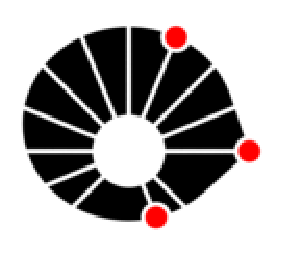
\includegraphics[scale=0.3]{LRCgraphics/logo-unicamp.eps}\\
    \textsc{
        Universidade Estadual de Campinas\\
        Instituto de Computação\\\vspace{-0.1cm}
        Laboratório de Redes de Computadores
    }
}

\date{Campinas, \today}

%-------------------------------------------------------
% THE BODY OF THE PRESENTATION
%-------------------------------------------------------

\begin{document}

%-CAPA
{\1
\begin{frame}[plain,noframenumbering]
\titlepage 
\end{frame}
}

%-AGENDA
\begin{frame}{Agenda}{}
    \tableofcontents
\end{frame}

%Aparece menu a cada nova seção
\AtBeginSection[]
{
    \begin{frame}<beamer>
    \frametitle{Agenda}
    \tableofcontents[currentsection]
    \end{frame}
}

%-INICIO
\section{Introdução}

%-
\subsection{Histórico}
\begin{frame}{Introdução}{Histórico}
    \begin{itemize}
        \item \textbf{1G}: Sistemas analógicos. Nenhum tipo de transmissão de pacotes de dados.
        \item \textbf{2G}: Sistemas digitais. Mensagens SMS, email, dentre outros. Taxas de transmissão de 9,6 kbps.
        \item \textbf{3G}: Sistemas celulares com serviços de dados por pacotes e taxas maiores que 256 kbps.
        \item \textbf{4G}: Sistemas projetados para oferecer taxas de download de 100Mbps com o usuário em movimento e 1Gbps com usuário parado. O uplink é de até 500Mbps.
        \item \textbf{5G}: Novas aplicações.
    \end{itemize}
\begin{figure}[!htb]
    \centering
    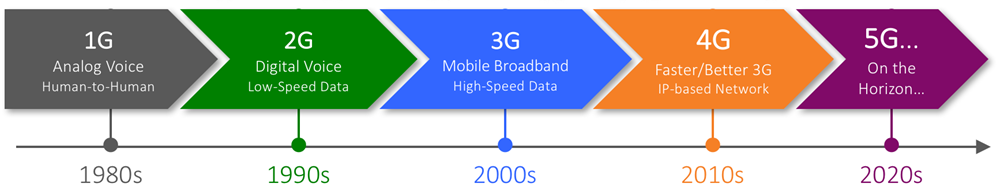
\includegraphics[scale=0.4]{images/5G-Evolution-Chart.png}
    \caption{Geração das redes móveis \cite{ciena5g2018}}
\end{figure}
\end{frame}

%-
\begin{frame}{LTE cont.}{Comutação}
\begin{table}[]
\begin{tabular}{l|l|l}
\hline
\textbf{Item} & \textbf{Circuitos} & \textbf{Pacotes} \\ \hline
Configuração de chamadas          & Obrigatória                     & Não necessária                \\ \hline
Caminho físico dedicado           & Sim                             & Não                           \\ \hline
Pacotes seguem o mesmo caminho    & Sim                             & Não                           \\ \hline
Pacotes chegam na mesma ordem     & Sim                             & Não                           \\ \hline
Reserva da largura de banda       & Fixa                            & Dinâmica                      \\ \hline
Largura de banda desperdiçada     & Sim                             & Não                           \\ \hline
A falha de um equipamento é fatal & Sim                             & Não                          \\ \hline
\end{tabular}
\caption{Comparação entre comutações de circuitos e pacotes\footnote{\url{http://www.teleco.com.br/tutoriais/tutorialvoipconv}}}
\end{table}
\end{frame}

%-
\begin{frame}{LTE}{Características}
\begin{table}[]
\begin{tabular}{l|l|l|l}
%\hline
Tecnologia      & Downlink\footnote{ERB $\rightarrow$ Celular} & Uplink\footnote{Celular $\rightarrow$ ERB}   & Canalização (MHz) \\ \hline
LTE             & 100 Mbps & 50 Mbps  & 20                \\ \hline
LTE-A           & 1.0 Gbps & 0.5 Gbps & 100               \\ \hline
LTE-A Pro       & 3.0 Gbps & 1.5 Gbps & 640               \\
%\hline
\end{tabular}
\caption{Principais características das redes LTE}
\end{table}

\end{frame}

%-
\section{Características}
\begin{frame}{LTE}{Características}
    \begin{itemize}
        \item Altas taxas de dados.
        \item Baixa latência.
        \item Comunicação de voz por IP, denominado VoIP.
        \item Utiliza OFDMA (Orthogonal Frequency Division Multiple Access) para Downlink.
        \item Utiliza SC-FDMA (Single Carrier - Frequency Division Multiple Access) para o Uplink.
    \end{itemize}
\end{frame}
%-
\begin{frame}{LTE}{Características}
    \begin{itemize}
        \item Altas taxas de dados.
        \item Baixa latência.
        \item Comunicação de voz por IP, denominado VoIP.
        \item Utiliza OFDMA (Orthogonal Frequency Division Multiple Access) para Downlink.
        \item Utiliza SC-FDMA (Single Carrier - Frequency Division Multiple Access) para o Uplink.
        \item Tecnologia de antena MIMO (Multiple Input Multiple Output).
        \item Infraestrutura simplificada, com dois tipos de nós: Estação Base e Gateways.
    \end{itemize}
\end{frame}

%-
\section{Seção 3}
\begin{frame}{LTE}{Arquitetura}
\begin{figure}[!ht]
	\centering
	\subfigure[Com contenção]{
	    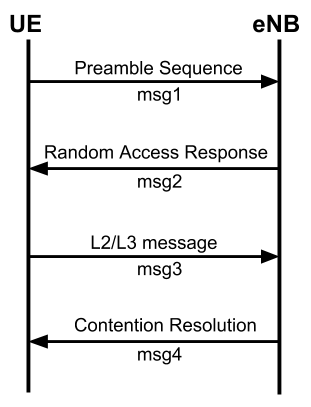
\includegraphics[scale=0.3]{images/contencao-based.png}
	}
	\subfigure[Sem contenção]{
	    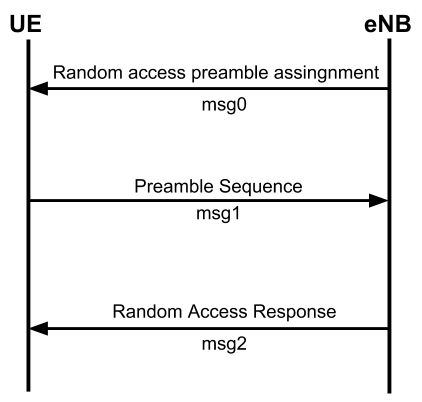
\includegraphics[scale=0.3]{images/contencao-free.png}
	}
	\label{fig:redecomplexa}
\end{figure}
\end{frame}

%- REFERENCIAS
\begin{frame}[allowframebreaks]{Referências}
\small{
    \bibliography{referencias}
}
\bibliographystyle{IEEEtran}
\end{frame}

%- FINAL
{\1
\begin{frame}[plain,noframenumbering]
  \finalpage{\large{
  \textbf{Obrigado!} \\
  \vspace{0.2cm}
  \url{www.lrc.ic.unicamp.br/~seuusuario}
  }}
\end{frame}
}

\end{document}